% Chapter 5
% add following line for typesetting from subfiles
% !TeX root = ../uet_thesis.tex
% !TeX root = ../uet_thesis.bbl
% !TeX root = ../references.bib
\chapter{Implementation and Performance Evaluation} % Write in your own chapter title
\label{Chapter6}
\lhead{Chapter 6. \emph{Implementation and Performance Evaluation}} % Write in your own chapter title to set the page header
%\section{Introduction}


%5)	Implementation and performance evaluation (Harsware + Error Probability)
%i)	Transmitter
%ii)	Receiver
%iii)	Practical results: P_e Vs Brightness Index
%iv)	Maximization Problem

%%%\section{Data Transmission Rate}
%%%The information carrying capacity of the proposed codes is affected by the selection of the codeword. A larger code size ensures more brightness levels and better information carrying capacity per symbol frame. In this section we would see the effect of codeword size and brightness index on information carrying capacity of the VR-MPPM codes.
%%%
%%%The code rate varies when brightness index is changed. Code rate is minimum for $r=1$ and $r=n-1$. The former case is the simple pulse position modulation encoding that provides effective code rate of $\lfloor \frac{1}{n} \log_2 \binom{n}{1} \rfloor$ while the later is the inverted pulse position modulation. Its code rate is same as that of PPM however it drives the light source at illumination level near peak value. Maximum data rate is achieved when brightness index is $0.50$ that is $r=\frac{n}{2}$ giving effective code rate value of $\lfloor \frac{1}{n} \log_2 \binom{n}{n/2} \rfloor$.  The relationship of the two parameters with frame size, plotted in figure \ref{fig:coderate_limits}, provides important insight for system design. It can be observed that the code efficiency decreases at lower brightness indices when frame size is increased. However the maximum code rate improves with larger frame size. It tends to approach unity as frame size is increased.
%%%
%%%The code-rate for brightness index = 0.5 can be applied in other line coding applications as well. In those cases the VR-MPPM code ensures $50\%$ duty cycle over one symbol frame that provides DC null and code transparency. The maximum number of consecutive ones or zero's comes out to be $2(n-1)$ in this case. The code rate will be about doubled as compared to Manchester or phase encoding.
%%%
%%%\begin{figure}[!htbp]
%%%	\centering
%%%	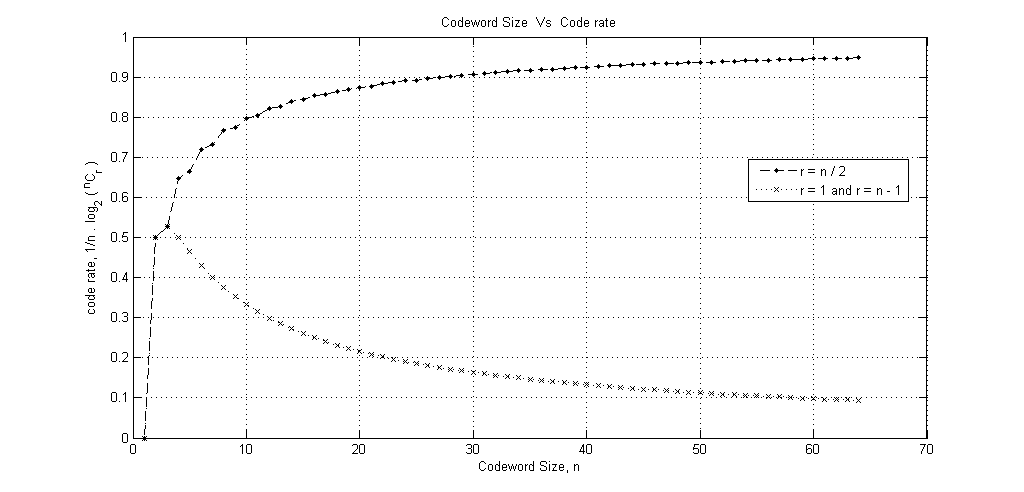
\includegraphics[width=\textwidth]{./Figures/max_min_coderate.png}
%%%	\caption[Coderate limits imposed by $n$]{Upper and lower limits on coderate as function of frame size, n}
%%%	\label{fig:coderate_limits}
%%%\end{figure}
%%%
%%%One more interesting result is the relation ship between data transmission rate versus the brightness index. The graph in figure \ref{fig:coderate_brightness} plots the code rate curves for different values of frame size. A curve for fixed $n$ is bell shape that results from the combinatorial mathematics relationship which states  $\binom{n}{r}=\binom{n}{n-r}$. It shows that the selection of larger frame size does not improve code rate by large degrees for brightness indices near the extreme values.
%%%
%%%\begin{figure}[!htbp]
%%%	\centering
%%%	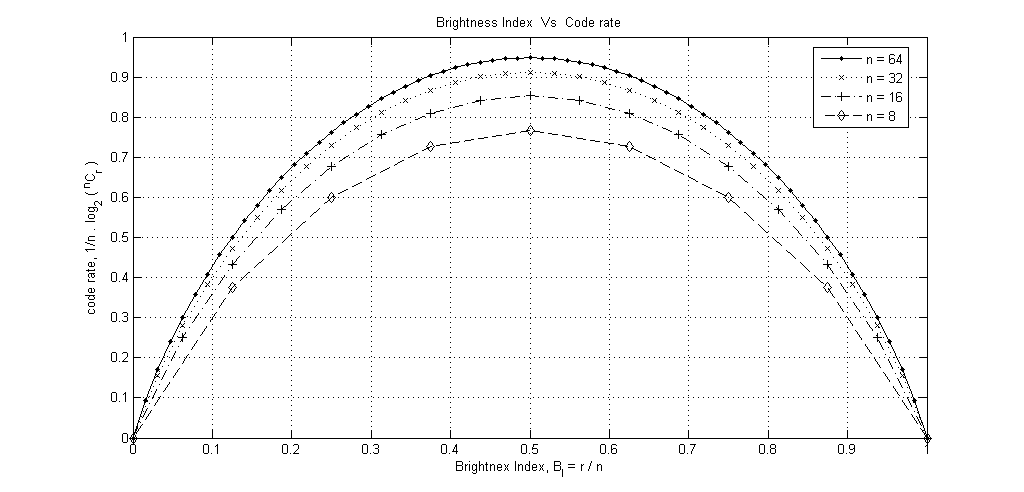
\includegraphics[width=\textwidth]{./Figures/coderate_brightness.png}
%%%	\caption{Dependence of code-rate on brightness index}
%%%	\label{fig:coderate_brightness}
%%%\end{figure}
%%%
%%%
%%%\section{Optimal Frame Size And Channel Conditions}
%%% It has been discussed earlier that both the brightness resolution and information carrying capacity of the VR-MPPM code improve when frame size is increased. However the symbol error probability increases, too, with the number of bits per frame, $n$. Therefore the frame size can not be increased arbitrarily. The effect can be observed by the relation between the single bit error probability, $p_e$ and the symbol decoding error probability, $p_s$ given be equation \ref{eq:error_probability}:
%%%
%%%\begin{equation}
%%%p_s=\left[1-(1-p_e)^n \right]
%%%\label{eq:error_probability}
%%%\end{equation}
%%%
%%%The probability of correctly detection of a symbol, given be the equation \ref{eq:correction_probability}, decreases with frame size n. The parameter $p_{s,corr}$ is plotted for two different values of single bit error probability $p_e$ in figure \ref{fig:symbol_error}
%%%
%%%\begin{equation}
%%% p_{s,corr}=\bar{p}_s=(1-p_e)
%%%\label{eq:correction_probability}
%%%\end{equation}
%%%
%%%\begin{figure}
%%%	\centering
%%%	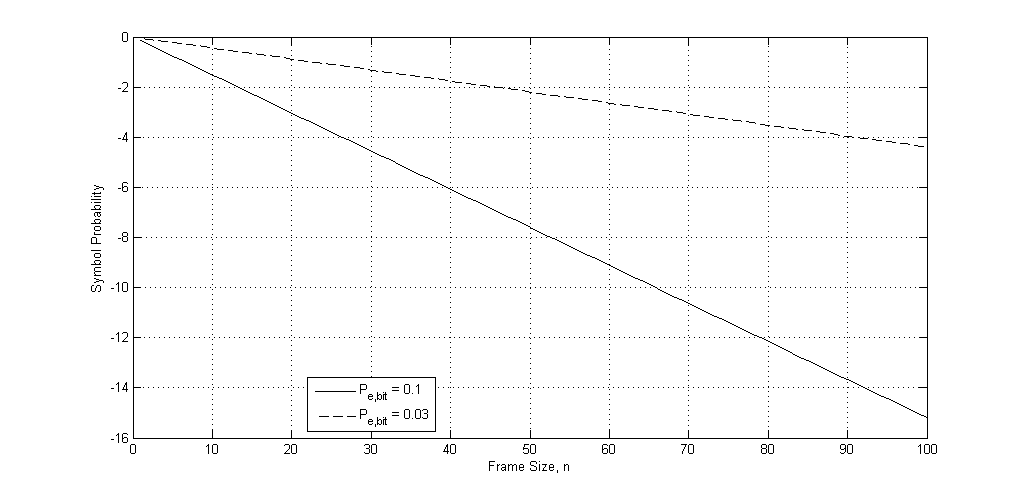
\includegraphics[width=\textwidth]{./Figures/SymbolVsn.png}
%%%	\caption[Symbol correctly decoding probablity]{Symbol correctly detection probability as a function of frame size}
%%%	\label{fig:symbol_error}
%%%\end{figure}
%%%
%%%These contradictory requirements point towards finding an optimal size of the codeword such that the brightness resolution and symbol correctly detection probability $p_{s,corr}$ are maximum possible. It leads to the evaluation of the optimization problem defined by equation \ref{eq:objective_function}. The objective function is plotted for two bit error probabilities in figure \ref{fig:objective_function}. Peak values in the graph indicate the optimal frame size for a given value of $p_e$
%%%\begin{figure}
%%%	\centering
%%%	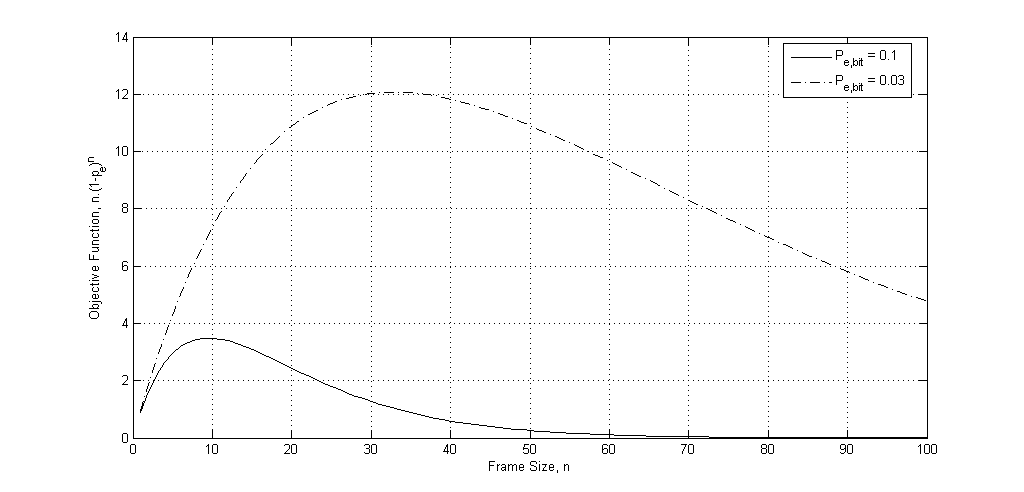
\includegraphics[width=\textwidth]{./Figures/ObjectiveFunction.png}
%%%	\caption{Encoder frame size objective function}
%%%	\label{fig:objective_function}
%%%\end{figure}
%%%
%%%\begin{equation}
%%%\begin{array}{cc}
%%%\mathbf{maximize}& f(n)=n(1-p_e)^n \\
%%%\mathbf{subject~to}& 0<n, 0 \leq p_e \leq 1
%%%\end{array}
%%%\label{eq:objective_function}
%%%\end{equation}
%%%
%%%The value of $n$ in equation \ref{eq:objective_function} can be relaxed to be a positive integer as it defines the number of bits in a codeword. The check for global optimality of the solution given by objective function, we take its second derivative given as
%%%
%%%\begin{equation}
%%%f''=(\bar{p}_e)^n \ln (\bar{p}_{s,corr})(n \ln \bar{p_e} + 2)
%%%\label{eq:second_d}
%%%\end{equation}
%%%
%%%Where $\bar{p}_e=(1-p_e)$ in equation \ref{eq:second_d}. The objective function based upon \ref{eq:second_d} comes out to be
%%%
%%%\begin{equation}
%%%    f(n) = \left\{\begin{array}{cccc}
%%%    concave & as~ f''(n) \leq 0  & for & \frac{2}{|\ln (1-p_e)|} \geq n \\
%%%    convex & as~ f''(n) \geq 0  & for & \frac{2}{|\ln (1-p_e)|} \leq n
%%%\end{array}   \right..
%%%\label{eq:concavity}
%%%\end{equation}
%%%
%%%The solution for equation \ref{eq:objective_function} evaluates to be
%%%
%%%\begin{equation}
%%%\psi (n) = \frac{1}{n}
%%%\end{equation}
%%%
%%%The optimality function $\psi(n)$ is plotted as a function of channel bit transitional probability $p_e$ in figure \ref{fig:optimal_function}
%%%
%%%
%%%\begin{figure}
%%%	\centering
%%%	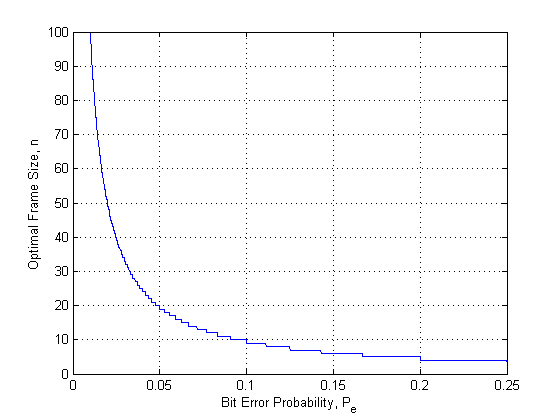
\includegraphics[width=\textwidth]{./Figures/OptimalFunction.png}
%%%	\caption{Optimal value of frame size Vs Bit transition probability}
%%%	\label{fig:optimal_function}
%%%\end{figure}

\section{Hardware Implementation}
Effectiveness of the proposed VR-MPPM line code is demonstrated by hardware implementation. A light source consisting of white LED grid is used as data transmitter paired with a receiver based upon an integrated photosensor module. The visible light wireless link is tested on two different platforms. The first implementation uses UART protocol to drive the light source. Serial port of a personal computer directly drives the LED circuit. The data bits in a UART packet are treated as one frame of VR-MPPM. Similarly at receiver end the photosensor module also directly connects to the PC serial port. The second implementation uses an FPGA board, Digilent Nexys-2\cite{nexys2}, and provides more freedom in selection of clock speed and frame size. Error performance of the visible light wireless link is evaluated by cycling through all possible codewords.

\section{UART Based Implementation}
The visible light wireless transmission implements VR-MPPM line code using byte frame of UART communication protocol. A USB to UART cable is used to interface the transmitter and receive modules to the computer. The converter cable is based upon Texas Instruments chip TUSB3410\cite{TUSB3410} that supports data speeds upto 921600 baud. The transmitter consists of 84 high brightness white LEDs mounted in grid form of $6\times 14$ LED. 14 LED are connected in parallel in a string. Three such strings are connected in series connection to form a $3\times 14$ LED bank. That means a bank of LEDs can be lighted from a 12V DC wall adapter. Two such banks are connected in parallel in the transmitter shown in figure \ref{fig:tx_hardware}. Texas Instruments' half-bridge bipolar switching integrated circuit UC2950T \cite{UC2950} is used as power driver.

\begin{figure}[hbtp]
\centering
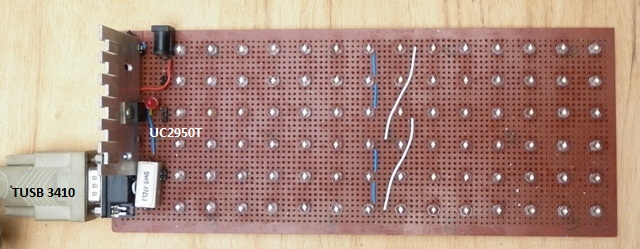
\includegraphics[angle=0,width=0.9\textwidth]{./Figures/Transmitter.jpg}
\caption[VLC transmitter hardware]{VLC transmitter light consists of 84 High brightness White light LED}
 \label{fig:tx_hardware}
\end{figure}

The receiver module is built around toshiba TORX173 \cite{TORX173} optical fiber receiver for digital audio. This particular module is radily available in the local market. It provides clean TTL electrical output signal  that is stabilized over wide range of optical signal power levels. This makes the interfacing with TUSB3410 \cite{TUSB3410}, USB to UART converter, hassle free. The optical receiver module supports data rates upto 6MHz that covers full range of the converter and LED driver chips. Receiver module is shown in figure \ref{fig:rx_hardware}. 

\begin{figure}[hbtp]
\centering
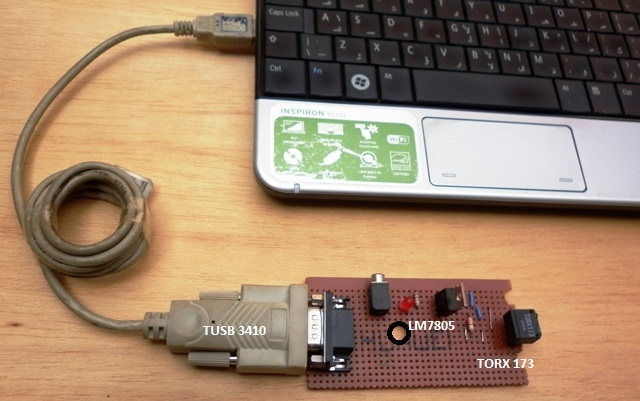
\includegraphics[angle=0,width=0.75\textwidth]{./Figures/Receiver_v2.jpg}
\caption[VLC receiver hardware]{VLC receiver built around Toshiba TORX173 integrated optical receiver module}
\label{fig:rx_hardware}
\end{figure}

UART based implementation is easier to setup as this protocol has been a classic data interfacing scheme and is already supported by a large number of devices. However brightness resolution is limited in this implementation. There are always two extra start and stop bits in a UART frame, inserted for synchronization. Therefore the dimming range is limited from $10\%$  to $90\%$ of the full brightness level.


%The hardware setup is used to evaluate the symbol error probability at different brightness indices. The graph in figure \ref{fig:evaluation1_hardware} shows the relationship. It is observed that minimum symbol error rate is achieved at around $0.5$ brightness index. Beyond that point on either side error probability is higher due to saturation of the receiver owing to unbalanced one-zero stream.
%\begin{figure}
%	\centering
%	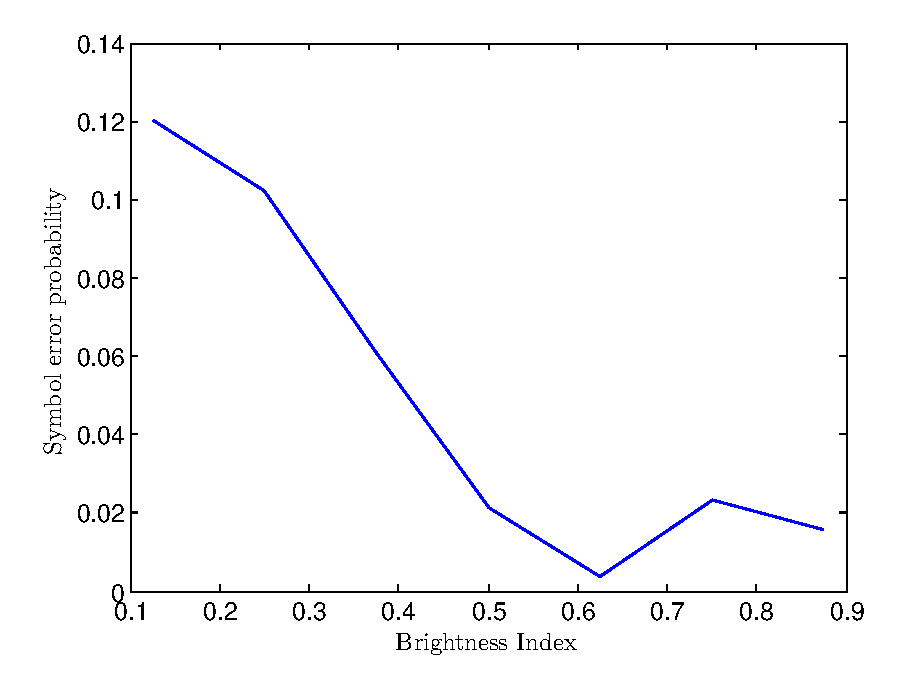
\includegraphics[width=\textwidth]{./Figures/experiment_brightness}
%	\caption[Effect of brightness index on symbol error rate]{Practical evaluation: Effect of brightness index on symbol error rate}
%	\label{fig:evaluation1_hardware}
%\end{figure}


\section{FPGA implementation on Xilinx Spartan-3 board}

The second performance test of the proposed VR-MPPM was evaluated on FPGA boards. This implementation was used to evaluate the data rate and error performance of the proposed codes over wider range of frame size and brightness indices. This implementation provided better control over brightness level along with faster data transmission as compared to the UART implementation. The prototype was setup in loop-back fashion with both the encoder and the decoder implemented on same Nexys-2 \cite{nexys2} FPGA board. This board hosts Xilinx Spartan 3E-500 FG320 FPGA chip.  Verilog Hardware Description Language (HDL) was used to implement the logic for VR-MPPM encoder, decoder and performance evaluation logic. Hardware is described at behavioural level therefore there is no significant difference between the earlier listed algorithms \ref{algo:Encoder} \ref{algo:Decoder} in Chapter-3 and the Verilog HDL code.

The LED light is operated at 500kHz clock. The brightness resolution (frame size) and brightness index are selectable from FPGA board. The test is performed by transmitting $10^6$ frames, cycling through all valid codes for the selected frame size and brightness index, and erroneous symbols are counted on the receiver. Symbol error probability is calculated as ratio of symbol error count and total transmitted symbols.
%\begin{figure}[hbtp]
%\centering
%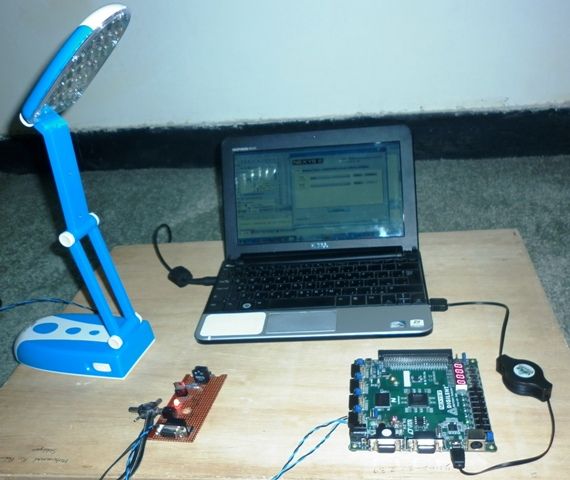
\includegraphics[angle=0,width=0.75\textwidth]{./Figures/Lamp_Off.jpg}
%%\caption{VLC setup with Nexys-2 Development Board}
%\label{fig:VLCNexys2On}
%\end{figure}
%
%
%\begin{figure}[hbtp]
%\centering
%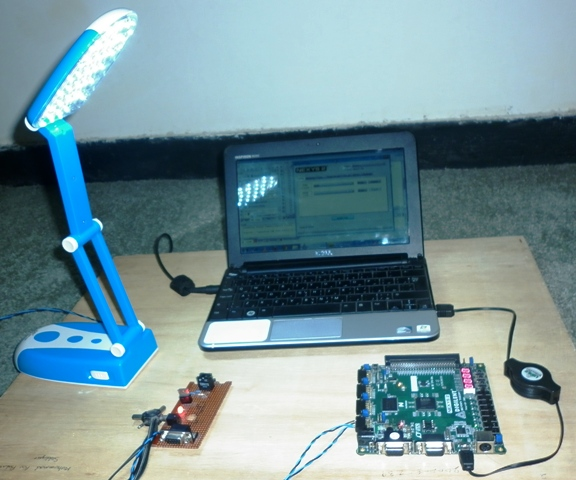
\includegraphics[angle=0,width=0.75\textwidth]{./Figures/Lamp_On.jpg}
%\caption{VLC setup with Nexys-2 Development Board}
%\label{fig:VLCNexys2Off}
%\end{figure}



\begin{figure}[hbtp]
\centering
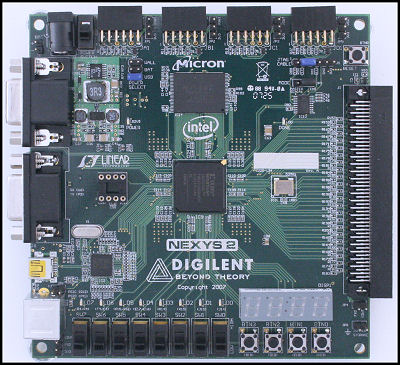
\includegraphics[angle=0,width=0.75\textwidth]{./Figures/NEXYS2_400.jpg}
\caption{Nexys-2 Development Board}
\label{fig:nexy2}
\end{figure}

\subsection{Encoder Module}
The encoder module implements the hardware description of algorithm \ref{algo:Encoder} presented in Chapter \ref{Chapter3}. It requires 'n' clock cycles to convert the input symbol $m$ to n-bit codeword, with $n$ defined by the signal $frameSize$. The combinatorial function $\binom{n}{r}$ is required by the encoder that is implemented using lookup table technique. This table is accessed using a separate \textbf{nCrROM} module that is listed in appendix \ref{sec:nCrROM}. The encoder evaluates most significant bit first and provides encoded data both in serial and parallel formats. Encoding process is started by a high level on $start$ input at positive clock edge. The $complete$ signal is asserted after encoding process is finished. The calculated codewords contains $r$ 1's in the output signal $out$.
\begin{figure}[!htbp]
	\centering
%	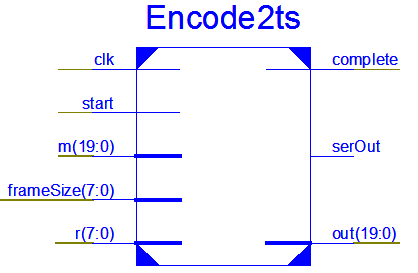
\includegraphics{./Figures/Encode2ts.png}
	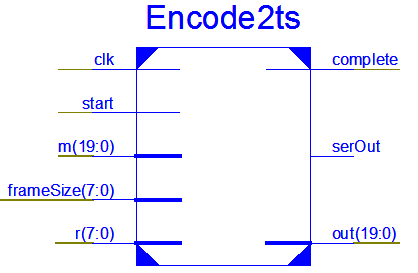
\includegraphics[width=.5\textwidth]{./Figures/Encode2ts.png}
	\caption{VR-MPPM encoder module}
	\label{fig:Encode2ts}
\end{figure}
\subsection{Decoder Module}
Decoder is implemented using algorithm \ref{algo:Decoder} in \ref{Chapter3}. This module also requires 'n' clock cycles to convert the n-bit input codeword back to the original symbol, evaluating the most significant bit first. Therefore encoder and decoder module can be made to work in back to back fashion with a serial link. In present implementation decoder takes in the codeword as a parallel input $m$. It is read at positive clock edge after the $start$ signal is set. Rest of the signals have same functionality as defined in encoder module.

\begin{figure}[!htbp]
	\centering
%	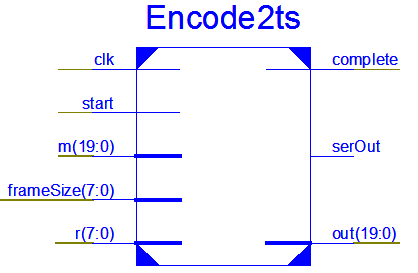
\includegraphics{./Figures/Encode2ts.png}
	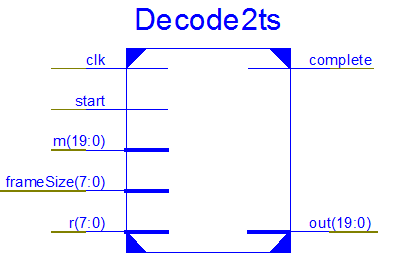
\includegraphics[width=.5\textwidth]{./Figures/Decode2ts.png}
	\caption{VR-MPPM decoder module}
	\label{fig:Decode2ts}
\end{figure}

\subsection{Parallel to Serial and Serial to Parallel (p2p) Module}
It is an intermediate module between encoder and decoder modules. Its role is to transmit and receive parallel data on an external serial link. The serial link consists of the visible light communication signal. To check the link performance of VR-MPPM at different frame sizes and brightness indices, serial data is sent out $serOut$ signal at positive clock edge that is read in through $serIn$ signal on negative edge of the clock. The signal $frameSize$ determines the frame size of serial output. The Nexys-2 boards' Pmod port $JA1$ is used to transmit and receives the data on serial link consisting of white LEDs and TORX-173 optical receiver. Verilog implementation of the module is listed in appendix \ref{sec:p2p}. The $clk$ input signal determines the bit time of the optical serial signal. This signal is helpful for evaluating code performance at different frequencies.
\begin{figure}[!htbp]
	\centering
	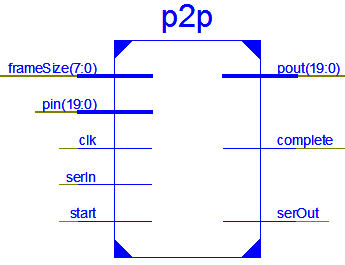
\includegraphics[width=.5\textwidth]{./Figures/p2p.png}
	\caption{Serial link module}
	\label{fig:p2p}
\end{figure}

%\subsection{Encoded Parallel$\leftrightarrow$Serial (ENp2p) Module}
\subsection{Encoded Parallel-Serial (ENp2p) Module}
This is an upper level module that integrates the encoder, p2p and encoder modules, thus completing the serial link with VR-MPPM encoded data. As encoder and decoder operate at primary clock frequency of the FPGA board, this module sets clock frequency suitable for white LED operation. The internal signal flow in this module takes place according to following sequence: Input word $pin$ is first encoded using encoder module \ref{sec:Encode2ts}. When this conversion is complete encoded word is sent over serial link using p2p module \ref{sec:p2p}. After parallel$\leftrightarrow$Serial$\leftrightarrow$Parallel through optical link operation is complete and serial data has been received completely, it is fed to the decoder module \ref{sec:Decode2ts}. Decoder module's $complete$ signal is asserted after all the three stages are completed.

\begin{figure}[!htbp]
	\centering
	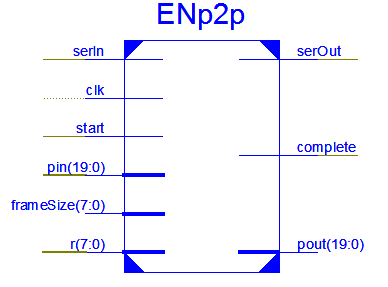
\includegraphics[width=.5\textwidth]{./Figures/ENp2p.png}
	\caption{VR-MPPM encoded serial link module}
	\label{fig:ENp2p}
\end{figure}

\subsection{Module for Scanning VLC Codes}
The scan codes \ref{sec:scanCodes} module is implemented to check the error rate performance of the optical link by cycling through all possible symbols for a particular selected frame size and brightness index. This module works on top of \textbf{ENp2p} module and keeps record of the errors encountered by comparing the received and transmitted symbols.

\begin{figure}
	\centering
	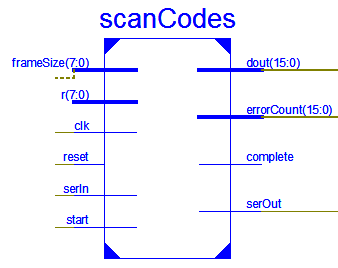
\includegraphics[width=.5\textwidth]{./Figures/scanCodes.png}
	\caption[Module for generating scan symbols]{Generate VR-MPPM symbols for onboard evaluation of bit error rate}
%	\caption{HDL block to generate, transmit and receive VR-MPPM symbols for onboard evaluation of bit error rate}
	\label{fig:scanCodes}
\end{figure}

\subsection{VLC Module}
VLC is the top level module. It defines the ports and signals of the Nexys-2 board that are used for external hardware intrfacing during actual functionality test. The user constraint file $toplevel.ucf$ \ref{sec:toplevel} defines the mapping of board ports to input\/output  signals.


%\begin{figure}[hbtp]
%\centering
%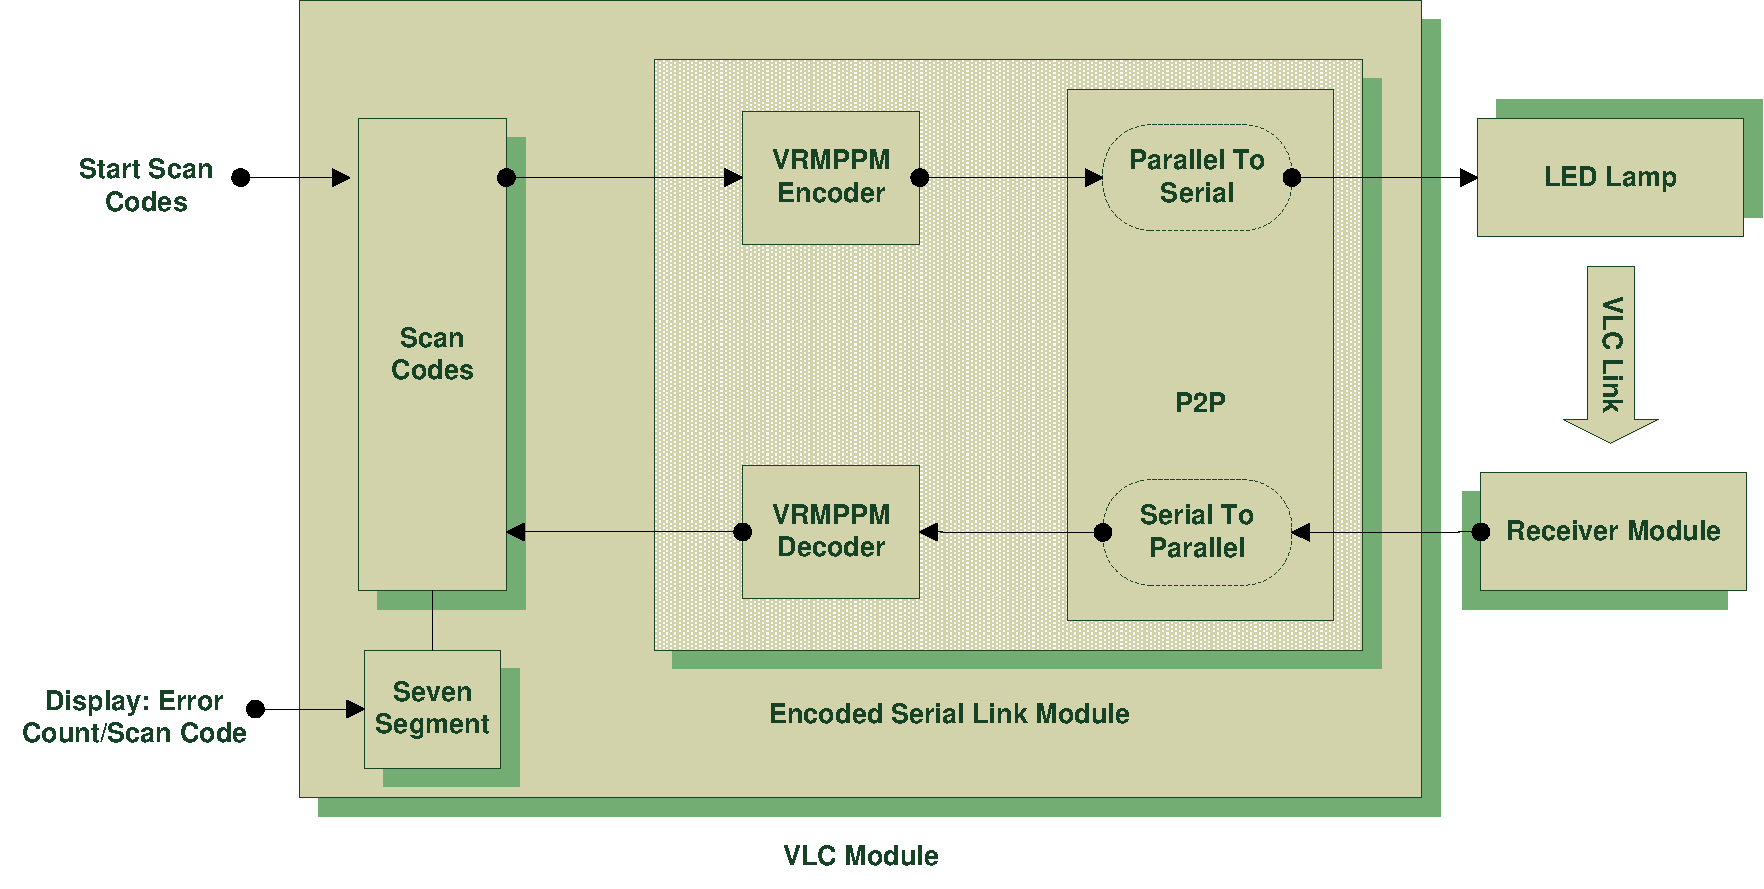
\includegraphics[angle=0,width=\textwidth]{./Figures/VLC_block_diagram}
%\caption{FPGA Implementation Block Diagram}
%\label{fig:FPGAblock}
%\end{figure}

%\subsection{User Constraints File}
%The constriant file \ref{sec:toplevel} for Nexys-2 board defines the pins used for VLC module signals.

\begin{figure}[!htbp]
	\centering
	\includegraphics[width=.5\textwidth]{./Figures/vlc.png}
	\caption[Toplevel VLC module]{HDL block diagram of top level module for serial link simulation}
	\label{fig:vlc}
\end{figure}

\subsection{Clock Divider Module}
The basic Nexys-2 board clock runs at 50MHz. This is too high frequency and is much higher than the capability of common available white LEDs. Therefore it is desired to divide down the origional clock to a transmitting frequency within few mega hertz. The clock divider module \textbf{clkDiv} takes in the system clock signal and outputs a new clock slowed down by the count value defined by the input word $newDiv$.

\begin{figure}[!htbp]
	\centering
	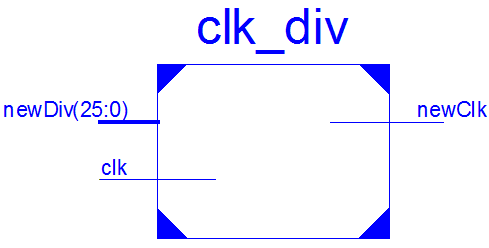
\includegraphics[width=.5\textwidth]{./Figures/clk_div.png}
	\caption[]{Clock divider module}
	\label{fig:clkDiv}
\end{figure}


\subsection{Seven Segment Driver Module} The Nexys-2 board houses a four digit seven segment display. This module drives the display to represent 16-bit word in hexadecimal format \ref{sec:LED_7seg}.

\begin{figure}[!htbp]
	\centering
	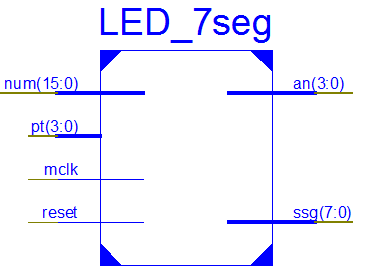
\includegraphics[width=.5\textwidth]{./Figures/LED_7seg.png}
	\caption{7-segment drivier module to display 16-bit values }
	\label{fig:LED_7seg}
\end{figure}

\section{Experimental Results}

The performance of a VR-MPPM visible light link at different brightness indices was evaluated using the FPGA platform. Transmitter and Receiver module were implemented on Digilent's Nexys-2 board. The transmitter consisted of off the shelf white LEDs. The receiver was built around TORX173 optical receiver module from Toshiba. Receiver and transmitter were interfaced to the Nexys-2 board using two interface lines of the $JA$ pmod connector. Symbol error rate was observed for three different values of frame size by varying the brightness index in the available range. The results are represented in figure \ref{fig:fpgaExperiment}. It can be observed that code error performance degrades for larger frame size at fixed brightness index, as depicted by equation \ref{eq:error_probability}.

\begin{figure}[!htbp]
	\centering
	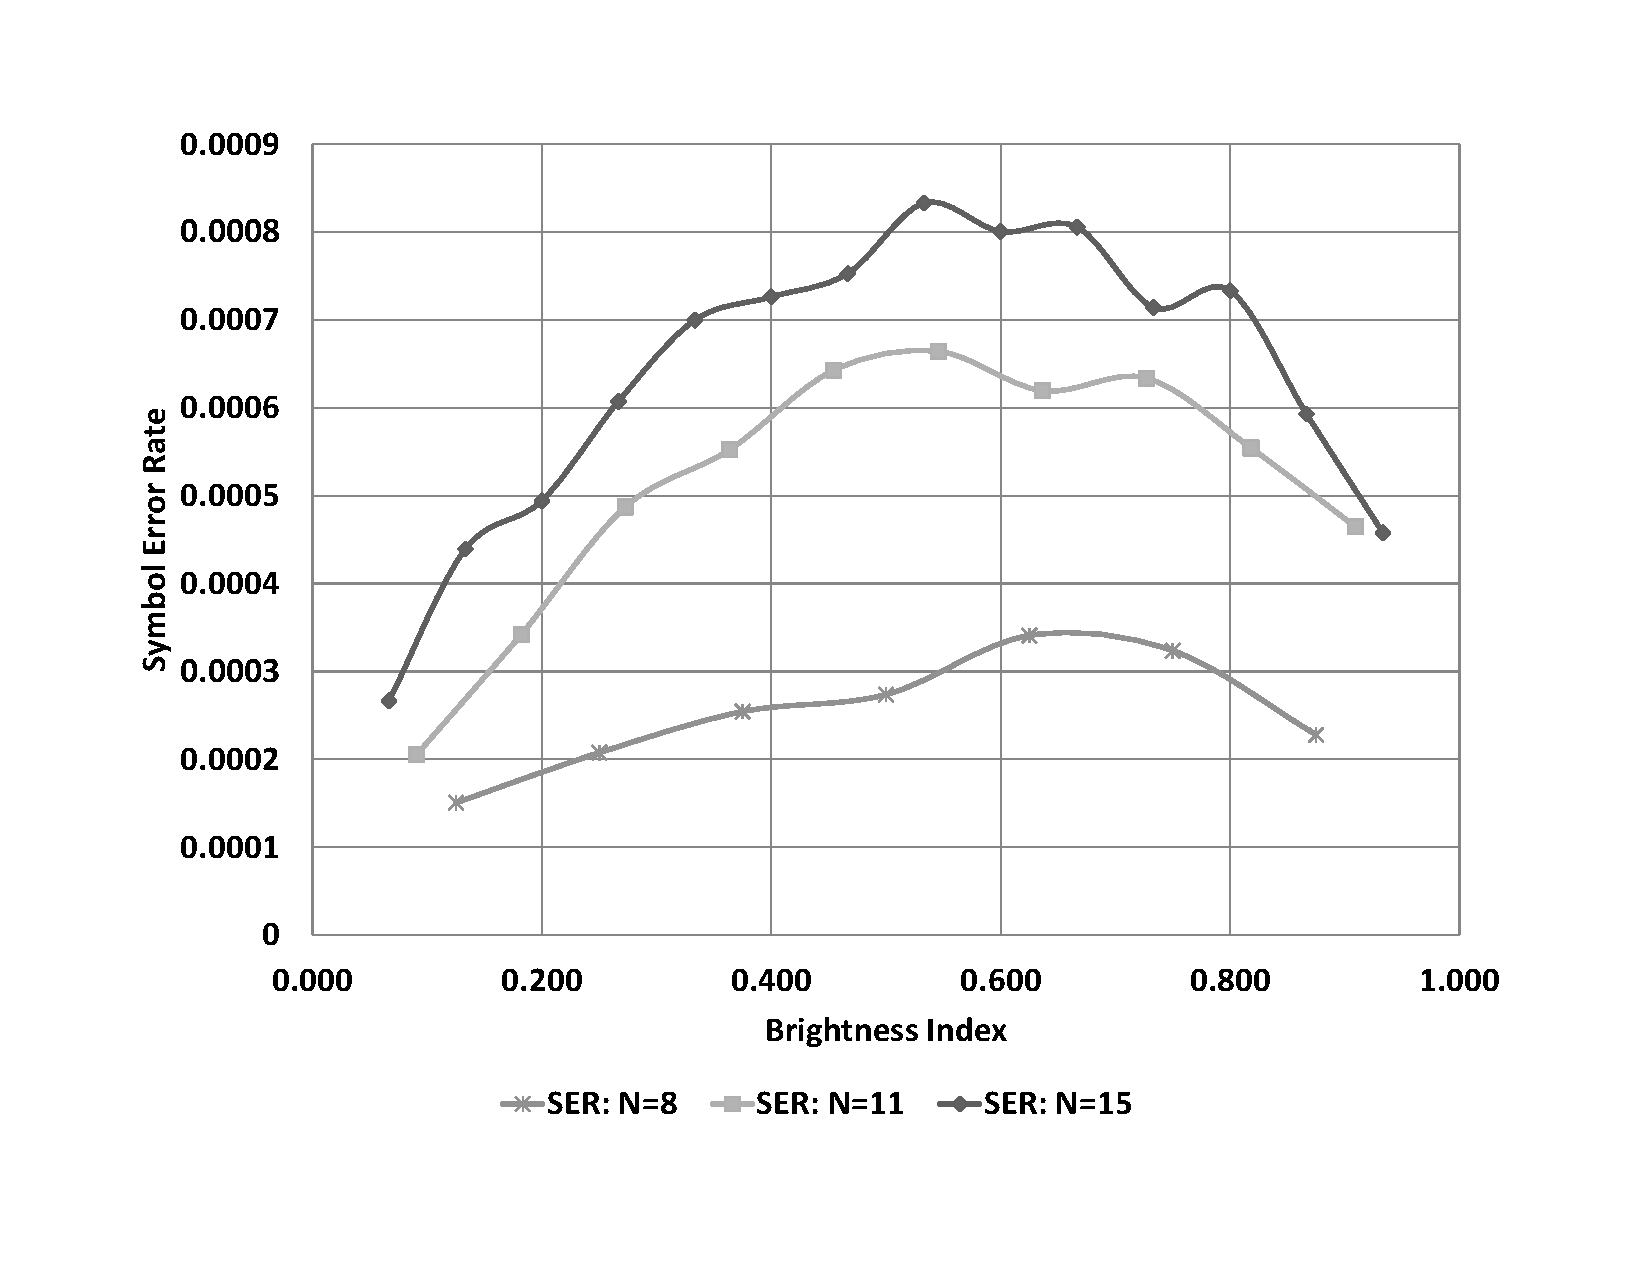
\includegraphics[width=0.8\textwidth]{./Figures/Experiment}
	\caption[Hardware Performance Evaluation]{Symbol error rate evaluation of VR-MPPM encoded symbols at different brigness indices. $n$ represents the frame size.}
	\label{fig:fpgaExperiment}
\end{figure}

For a given frame size, the symbol error rate curve takes a bell shaped curve with maximum number of errors encountered around 50\% brightness level. From discussion of the proposed VR-MPPM codes it is known that maximum bit transitions occur arround 50\% brightness as shown in figure \ref{Fig:line_codes2}. This is also the point for maxim data transmission rate and drive signal undergoes maximum number of transitions. The higher bandwidth requirement account for larger number of errors due to limited switching speed of the transmitter LED.
These experimental results are also in close agreement to the MPPM channel modelling presented in \cite{hamkins2005multipulse}. 

%
%Let $p_0(y)$ denotes the conditional probability of decoding a bit as 'y' when a zero was transmitted and $p_1(y)$ is the probability of decoding 'y' when a one was transmitted. Suppose in a frame size consisting of 'n' time slots of which first 'r' time slots contain a one and last 'n-r' slots contain a zero. Considering the discrete memory less channel with hard detection, the probability of decoding error of a symbol 's' is given by:
%
%\[
% P_{ser} = (probability~of~1\rightarrow 0~transition)^r \times  (probability~of~0\rightarrow 1~transition)^{n-r} 
%\]
%
%Now there are a total of $2^n$ codewords possible with $n$ slots. We need to calculate the probability for $\binom{n}{r}$ symbols in group of total possible symbols. It provides with the probability of symbol decoding error with $r$ ones as
%
%\[
% P_{ser,r} = \frac{1}{2^n} \binom{n}{r}(probability~of~1\rightarrow 0~transition)^r \times  (probability~of~0\rightarrow 1~transition)^{n-r} 
%\]
%
%
%\begin{equation}
% P_{ser,r} = \frac{1}{2^n} \binom{n}{r} p_1^r(0) \times  p_0^{n-r}(1) 
%\label{eq:ser2}
%\end{equation}
%
%Equation \ref{eq:ser2} hints at a bell shaped curve for symbol error rate performance.



\begin{figure}[!htbp]
\centering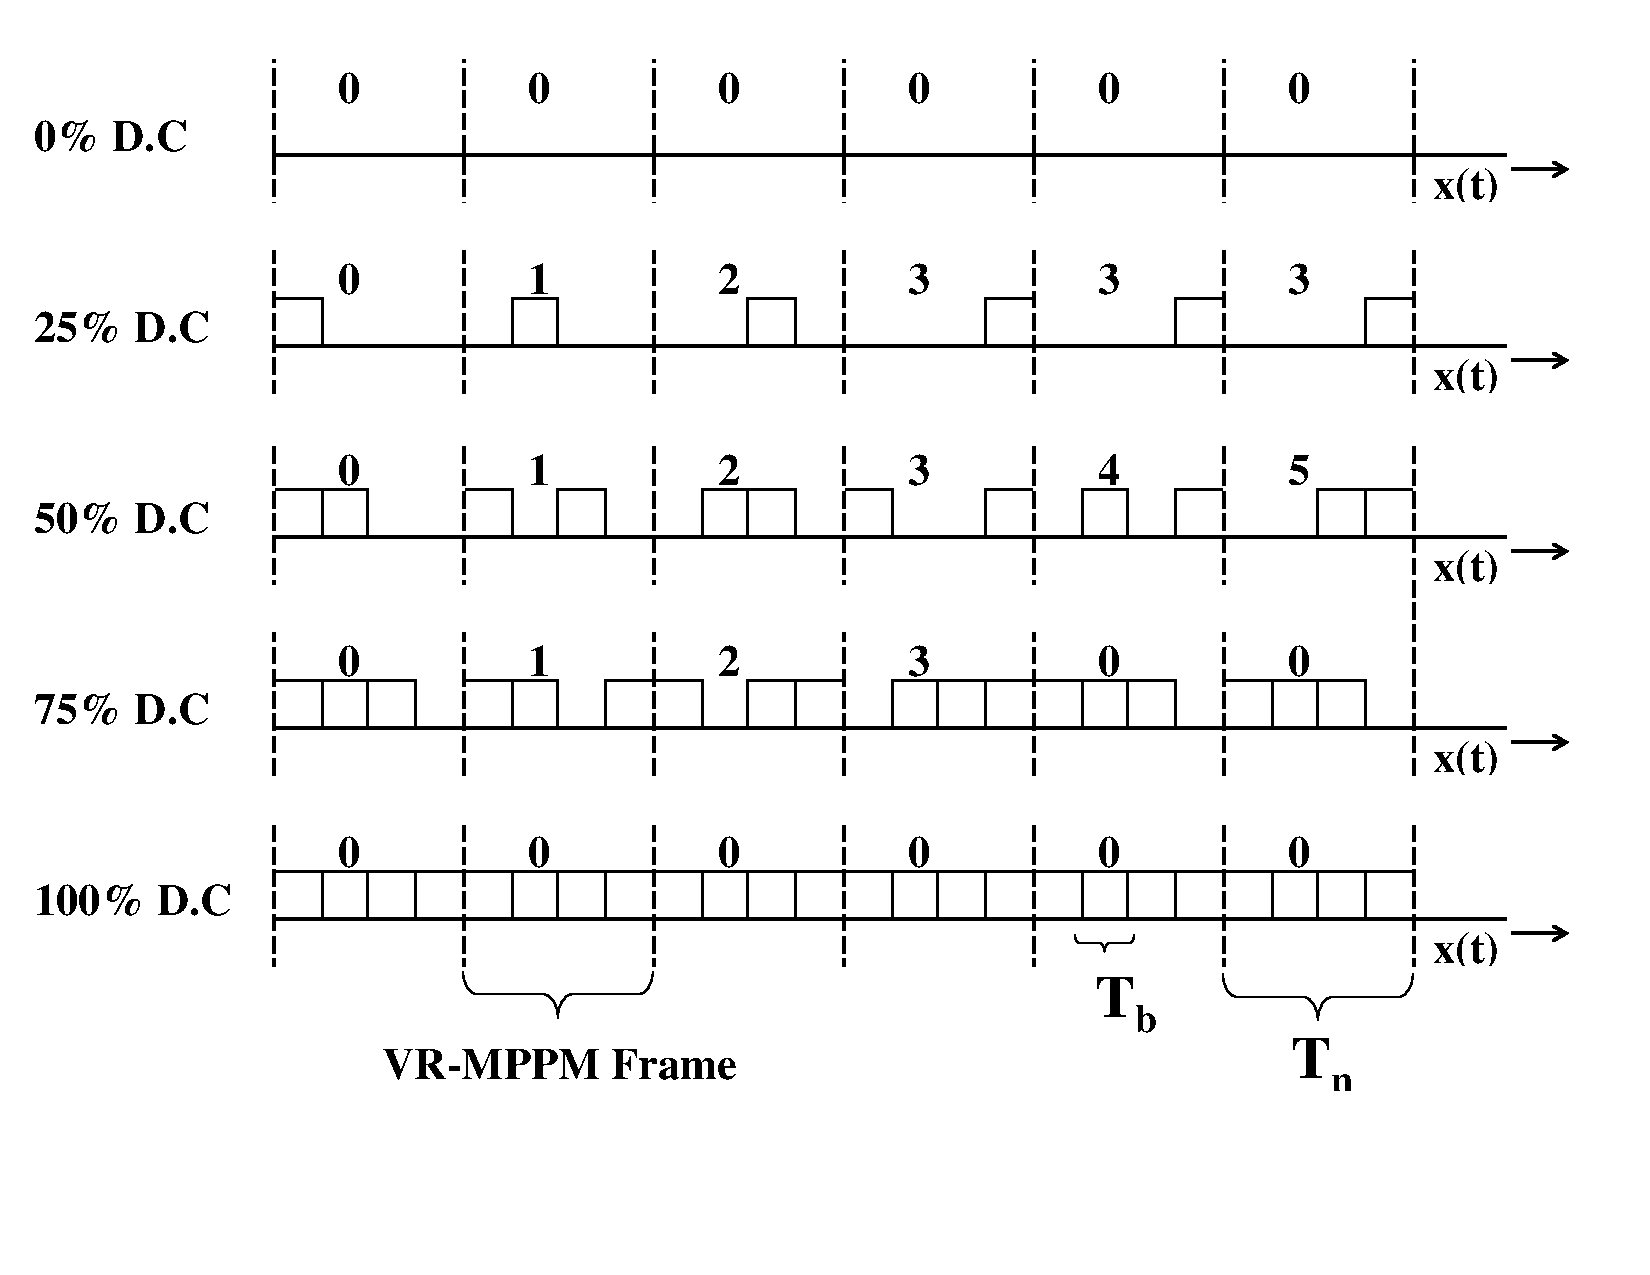
\includegraphics[width=0.8\textwidth]{./Figures/line_code}
\caption[VR-MPPM line waveforms]{VR-MPPM waveforms: Maximum transitions occur at 50\% brightness}
\label{Fig:line_codes2}
\end{figure}